% =========================================================================
% BÀI 12: BẢNG CỘNG, BẢNG TRỪ TRONG PHẠM VI 10 (CHỦ ĐỀ 3 - TOÁN LỚP 1)
% TOÀN BỘ CÂU HỎI ĐƯỢC VẼ HÌNH MINH HỌA TRỰC QUAN 100% BẰNG TIKZ
% =========================================================================

% --- CÁC HÀM VẼ SƠ ĐỒ VÀ ĐỒ VẬT TRỰC QUAN CHO BẢNG CỘNG TRỪ ---
\providecommand{\VeSoDoTachGop}[6]{% #1=x, #2=y, #3=tổng, #4=nhánh 1, #5=nhánh 2, #6=màu
  \begin{scope}[shift={(#1,#2)}]
    % Nhánh nối
    \draw[line width=1.5pt, #6!80!black] (0,0.8) -- (-1.1,-0.5);
    \draw[line width=1.5pt, #6!80!black] (0,0.8) -- (1.1,-0.5);
    % Vòng tròn tổng ở trên
    \draw[fill=#6!25, draw=#6!90!black, line width=1.4pt] (0,0.8) circle (0.55cm);
    \node[font=\large\bfseries\color{#6!95!black}] at (0,0.8) {#3};
    % Vòng tròn nhánh 1
    \draw[fill=yellow!35, draw=orange!90!black, line width=1.3pt] (-1.1,-0.5) circle (0.5cm);
    \node[font=\large\bfseries\color{orange!95!black}] at (-1.1,-0.5) {#4};
    % Vòng tròn nhánh 2
    \draw[fill=cyan!25, draw=blue!90!black, line width=1.3pt] (1.1,-0.5) circle (0.5cm);
    \node[font=\large\bfseries\color{blue!95!black}] at (1.1,-0.5) {#5};
  \end{scope}
}

\providecommand{\VeChuGaCon}[2]{% #1=x, #2=y
  \begin{scope}[shift={(#1,#2)}, scale=0.55]
    \fill[yellow!95!orange] (0,0) circle (0.22cm);
    \fill[yellow!95!orange] (0.12,0.18) circle (0.15cm);
    \fill[orange!95!black] (0.24,0.18) -- (0.38,0.14) -- (0.24,0.1) -- cycle;
    \fill[black] (0.16,0.21) circle (0.03cm);
    \fill[orange!90!black] (-0.08,-0.22) -- (-0.08,-0.32);
    \fill[orange!90!black] (0.08,-0.22) -- (0.08,-0.32);
  \end{scope}
}

\providecommand{\VeBongHoaNho}[3][magenta!80!red]{% #1=màu, #2=x, #3=y
  \begin{scope}[shift={(#2,#3)}, scale=0.55]
    \foreach \a in {0,72,144,216,288} {
      \fill[#1] (\a:0.18) circle (0.12cm);
    }
    \fill[yellow!95!orange] (0,0) circle (0.1cm);
  \end{scope}
}

% =========================================================================
% PHẦN 1: TRẮC NGHIỆM LỰA CHỌN (12 CÂU)
% =========================================================================
\textbf{Phần 1. Trắc nghiệm lựa chọn}
\setcounterpageref{ex}{0}

% --- CÂU 1 ---
\begin{ex} %[1D3N12]
Quan sát thanh mười ô gồm 4 chấm đỏ và 5 chấm xanh. Tính kết quả của phép cộng $4 + 5$:
\begin{center}
\begin{tikzpicture}[scale=0.75, baseline=(current bounding box.center)]
  \draw[fill=white, draw=blue!85!black, line width=1.4pt] (-2.75,-1.1) rectangle (2.75,1.1);
  \foreach \x in {-1.65, -0.55, 0.55, 1.65} {
    \draw[line width=1pt, blue!70!black] (\x,-1.1) -- (\x,1.1);
  }
  \draw[line width=1pt, blue!70!black] (-2.75,0) -- (2.75,0);
  
  % Hàng 1: 4 chấm đỏ
  \foreach \x in {-2.2, -1.1, 0, 1.1} {
    \fill[red!85!black] (\x,0.55) circle (0.33cm);
  }
  % Hàng 2: 5 chấm xanh
  \foreach \x in {-2.2, -1.1, 0, 1.1, 2.2} {
    \fill[cyan!75!blue] (\x,-0.55) circle (0.33cm);
  }
  \node[below=4pt, font=\small\bfseries\color{blue!90!black}] at (0,-1.2) {4 chấm đỏ $+$ 5 chấm xanh = ? chấm};
\end{tikzpicture}
\end{center}
\choice
{\True $9$}
{$8$}
{$10$}
{$7$}
\loigiai{
Ta có: $4 + 5 = 9$.\\
\textbf{Đáp án của câu hỏi là A}
}
\end{ex}

% --- CÂU 2 ---
\begin{ex} %[1D3N12]
Băng giấy có 10 ô vuông, bớt đi 3 ô bị gạch chéo. Tính kết quả của phép trừ $10 - 3$:
\begin{center}
\begin{tikzpicture}[scale=0.75, baseline=(current bounding box.center)]
  % 7 ô trắng còn lại
  \foreach \i in {0,1,2,3,4,5,6} {
    \draw[fill=white, draw=blue!85!black, line width=1.1pt] (\i*0.9 - 4.5, -0.45) rectangle (\i*0.9 - 3.6, 0.45);
    \node[font=\small\bfseries\color{blue!90!black}] at (\i*0.9 - 4.05, 0) {\pgfmathparse{int(\i+1)}\pgfmathresult};
  }
  % 3 ô gạch chéo
  \foreach \i in {0,1,2} {
    \draw[fill=gray!20, draw=gray!70!black, line width=1.1pt] (\i*0.9 + 1.8, -0.45) rectangle (\i*0.9 + 2.7, 0.45);
    \draw[line width=1.6pt, red!85!black] (\i*0.9+1.8,-0.45) -- (\i*0.9+2.7,0.45);
    \draw[line width=1.6pt, red!85!black] (\i*0.9+1.8,0.45) -- (\i*0.9+2.7,-0.45);
  }
  \node[below=4pt, font=\small\bfseries\color{blue!90!black}] at (-1.35,-0.55) {10 ô bớt 3 ô ($10 - 3 = ?$)};
\end{tikzpicture}
\end{center}
\choice
{$6$}
{$8$}
{\True $7$}
{$9$}
\loigiai{
Ta có: $10 - 3 = 7$.\\
\textbf{Đáp án của câu hỏi là C}
}
\end{ex}

% --- CÂU 3 ---
\begin{ex} %[1D3H12]
Quan sát sơ đồ tách - gộp số dưới đây. Từ phép cộng $4 + 6 = 10$, ta viết được hai phép trừ tương ứng là gì?
\begin{center}
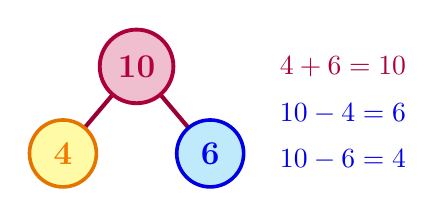
\begin{tikzpicture}[scale=0.85, baseline=(current bounding box.center)]
  \VeSoDoTachGop{0}{0}{10}{4}{6}{purple}
  \node[right=12pt, font=\normalsize\bfseries\color{purple!90!black}] at (1.5,0.8) {$4 + 6 = 10$};
  \node[right=12pt, font=\normalsize\bfseries\color{blue!90!black}] at (1.5,0.1) {$\implies 10 - 4 = 6$};
  \node[right=12pt, font=\normalsize\bfseries\color{blue!90!black}] at (1.5,-0.6) {$\implies 10 - 6 = 4$};
\end{tikzpicture}
\end{center}
\choice
{$10 - 2 = 8$}
{$10 - 5 = 5$}
{\True $10 - 4 = 6$ và $10 - 6 = 4$}
{$6 - 4 = 2$}
\loigiai{
Từ sơ đồ gộp 4 và 6 được 10, ta có hai phép trừ: $10 - 4 = 6$ và $10 - 6 = 4$.\\
\textbf{Đáp án của câu hỏi là C}
}
\end{ex}

% --- CÂU 4 ---
\begin{ex} %[1D3H12]
Quan sát sơ đồ tách - gộp số 8. Từ phép tính $3 + 5 = 8$, viết được hai phép trừ là:
\begin{center}
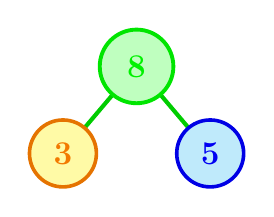
\begin{tikzpicture}[scale=0.85, baseline=(current bounding box.center)]
  \VeSoDoTachGop{0}{0}{8}{3}{5}{green}
\end{tikzpicture}
\end{center}
\choice
{$8 - 2 = 6$}
{\True $8 - 3 = 5$ và $8 - 5 = 3$}
{$8 - 4 = 4$}
{$5 - 3 = 2$}
\loigiai{
Từ $3 + 5 = 8$, ta viết được: $8 - 3 = 5$ và $8 - 5 = 3$.\\
\textbf{Đáp án của câu hỏi là B}
}
\end{ex}

\newpage
% --- CÂU 5 ---
\begin{ex} %[1D3H12]
So sánh hai vế phép tính: $3 + 7$ và $10 - 0$:
\begin{center}
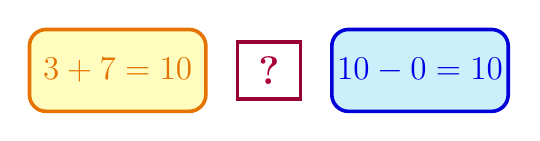
\begin{tikzpicture}[scale=0.8, baseline=(current bounding box.center)]
  % Khung vế trái
  \draw[fill=yellow!25, draw=orange!90!black, line width=1.3pt, rounded corners=6pt] (-3.8,-0.65) rectangle (-1.0,0.65);
  \node[font=\large\bfseries\color{orange!90!black}] at (-2.4,0) {$3 + 7 = 10$};
  
  % Ô điền dấu
  \draw[fill=white, draw=purple!80!black, line width=1.3pt] (-0.5,-0.45) rectangle (0.5,0.45);
  \node[font=\Large\bfseries\color{purple!90!black}] at (0,0) {?};
  
  % Khung vế phải
  \draw[fill=cyan!20, draw=blue!85!black, line width=1.3pt, rounded corners=6pt] (1.0,-0.65) rectangle (3.8,0.65);
  \node[font=\large\bfseries\color{blue!90!black}] at (2.4,0) {$10 - 0 = 10$};
\end{tikzpicture}
\end{center}
\choice
{$>$}
{$<$}
{Không so sánh được}
{\True $=$}
\loigiai{
Ta có: $3 + 7 = 10$ và $10 - 0 = 10$. Vì $10 = 10$ nên điền dấu $=$.\\
\textbf{Đáp án của câu hỏi là D}
}
\end{ex}

% --- CÂU 6 ---
\begin{ex} %[1D3H12]
Phép tính nào dưới đây có kết quả bằng 8?
\begin{center}
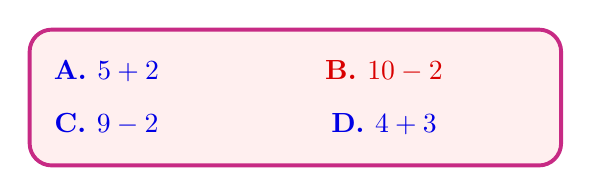
\begin{tikzpicture}[scale=0.75, baseline=(current bounding box.center)]
  \draw[fill=pink!25, draw=magenta!80!black, line width=1.4pt, rounded corners=8pt] (-4.5,-1.15) rectangle (4.5,1.15);
  \node[font=\normalsize\bfseries\color{blue!90!black}] at (-3.2,0.45) {A. $5 + 2$};
  \node[font=\normalsize\bfseries\color{red!85!black}] at (1.5,0.45) {B. $10 - 2$};
  \node[font=\normalsize\bfseries\color{blue!90!black}] at (-3.2,-0.45) {C. $9 - 2$};
  \node[font=\normalsize\bfseries\color{blue!90!black}] at (1.5,-0.45) {D. $4 + 3$};
\end{tikzpicture}
\end{center}
\choice
{\True $10 - 2$}
{$5 + 2$}
{$9 - 2$}
{$4 + 3$}
\loigiai{
Ta có: $10 - 2 = 8$. (Các câu khác: $5+2=7$, $9-2=7$, $4+3=7$).\\
\textbf{Đáp án của câu hỏi là A}
}
\end{ex}

% --- CÂU 7 ---
\begin{ex} %[1D3V12]
Quan sát sơ đồ tách - gộp số 9 dưới đây. Số thích hợp điền vào dấu hỏi chấm là:
\begin{center}
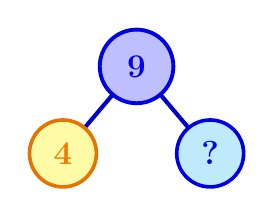
\begin{tikzpicture}[scale=0.85, baseline=(current bounding box.center)]
  \VeSoDoTachGop{0}{0}{9}{4}{?}{blue}
\end{tikzpicture}
\end{center}
\choice
{$4$}
{$6$}
{$3$}
{\True $5$}
\loigiai{
9 gồm 4 và 5: $9 - 4 = 5$.\\
\textbf{Đáp án của câu hỏi là D}
}
\end{ex}

% --- CÂU 8 ---
\begin{ex} %[1D3V12]
Chú ong mang phép tính nào dưới đây để bay về bông hoa mang số 10?
\begin{center}
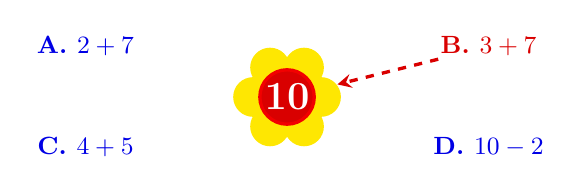
\begin{tikzpicture}[scale=0.8, baseline=(current bounding box.center)]
  % Bông hoa số 10 ở giữa
  \begin{scope}[shift={(0,0)}, scale=0.9]
    \foreach \a in {0,60,120,180,240,300} {
      \fill[yellow!90!orange] (\a:0.6) circle (0.35cm);
    }
    \draw[fill=red!85!black, draw=red!95!black, line width=1.2pt] (0,0) circle (0.48cm);
    \node[font=\Large\bfseries\color{white}] at (0,0) {10};
  \end{scope}
  
  % 4 phép tính xung quanh
  \node[font=\small\bfseries\color{blue!90!black}] at (-3.2,0.8) {A. $2 + 7$};
  \node[font=\small\bfseries\color{red!85!black}] at (3.2,0.8) {B. $3 + 7$};
  \node[font=\small\bfseries\color{blue!90!black}] at (-3.2,-0.8) {C. $4 + 5$};
  \node[font=\small\bfseries\color{blue!90!black}] at (3.2,-0.8) {D. $10 - 2$};
  
  \draw[->, >=stealth, dashed, line width=1.2pt, red!85!black] (2.4,0.6) -- (0.8,0.2);
\end{tikzpicture}
\end{center}
\choice
{$2 + 7$}
{\True $3 + 7$}
{$4 + 5$}
{$10 - 2$}
\loigiai{
Ta có: $3 + 7 = 10$. (Các phép tính khác: $2+7=9$, $4+5=9$, $10-2=8$).\\
\textbf{Đáp án của câu hỏi là B}
}
\end{ex}

\newpage
% --- CÂU 9 ---
\begin{ex} %[1D3V12]
Tính giá trị biểu thức gồm cả phép cộng và phép trừ: $6 + 3 - 4$.
\begin{center}
\begin{tikzpicture}[scale=0.8, baseline=(current bounding box.center)]
  \draw[fill=orange!15, draw=orange!90!black, line width=1.3pt, rounded corners=6pt] (-3.5,-0.6) rectangle (3.5,0.6);
  \node[font=\Large\bfseries\color{blue!90!black}] at (0,0) {$6 + 3 - 4 = ?$};
  \node[below=4pt, font=\small\bfseries\color{purple!85!black}] at (0,-0.65) {Thực hiện từ trái sang phải: $6 + 3 = 9$, rồi $9 - 4 = ?$};
\end{tikzpicture}
\end{center}
\choice
{$4$}
{$6$}
{\True $5$}
{$7$}
\loigiai{
Thực hiện từ trái sang phải: $6 + 3 = 9$; sau đó $9 - 4 = 5$.\\
\textbf{Đáp án của câu hỏi là C}
}
\end{ex}

% --- CÂU 10 ---
\begin{ex} %[1D3V12]
Quan sát chiếc cân đĩa thăng bằng dưới đây. So sánh hai vế: $10 - 5$ và $2 + 3$:
\begin{center}
\begin{tikzpicture}[scale=0.8, baseline=(current bounding box.center)]
  % Trụ cân
  \fill[gray!80!black] (-0.25,-1.2) rectangle (0.25,0);
  \fill[blue!90!black] (0,0) circle (0.15cm);
  \draw[fill=gray!60, draw=gray!90!black, line width=1pt] (-1.2,-1.4) rectangle (1.2,-1.15);
  \draw[line width=2.5pt, blue!90!black] (-3.0,0) -- (3.0,0);
  
  % Đĩa trái (10-5)
  \draw[line width=1pt, gray!70!black] (-3.0,0) -- (-3.8,-0.6);
  \draw[line width=1pt, gray!70!black] (-3.0,0) -- (-2.2,-0.6);
  \draw[fill=orange!25, draw=orange!90!black, line width=1.2pt] (-3.0,-0.6) ellipse (1.1cm and 0.25cm);
  \node[above=2pt, font=\small\bfseries\color{blue!90!black}] at (-3.0,-0.55) {$10 - 5 = 5$};
  
  % Đĩa phải (2+3)
  \draw[line width=1pt, gray!70!black] (3.0,0) -- (2.2,-0.6);
  \draw[line width=1pt, gray!70!black] (3.0,0) -- (3.8,-0.6);
  \draw[fill=orange!25, draw=orange!90!black, line width=1.2pt] (3.0,-0.6) ellipse (1.1cm and 0.25cm);
  \node[above=2pt, font=\small\bfseries\color{blue!90!black}] at (3.0,-0.55) {$2 + 3 = 5$};
  
  \node[below=4pt, font=\small\bfseries\color{purple!85!black}] at (0,-1.4) {Cân thăng bằng: $10 - 5 \dots 2 + 3$};
\end{tikzpicture}
\end{center}
\choice
{$>$}
{$<$}
{Không so sánh được}
{\True $=$}
\loigiai{
Ta có: $10 - 5 = 5$ và $2 + 3 = 5$. Vì $5 = 5$ nên điền dấu $=$.\\
\textbf{Đáp án của câu hỏi là D}
}
\end{ex}

% --- CÂU 11 ---
\begin{ex} %[1D3V12]
Một đàn gà có tất cả 10 con gồm gà trống và gà mái. Biết có 4 con gà trống, hỏi đàn gà có bao nhiêu con gà mái?
\begin{center}
\begin{tikzpicture}[scale=0.8, baseline=(current bounding box.center)]
  % Chuồng gà 10 con
  \draw[fill=green!12, draw=green!70!black, line width=1.3pt, rounded corners=8pt] (-4.2,-1.05) rectangle (4.2,1.05);
  % 4 gà trống
  \foreach \i in {0,1,2,3} {
    \VeChuGaCon{\i*0.9 - 3.4}{0.2}
  }
  \node[below=3pt, font=\small\bfseries\color{orange!90!black}] at (-2.05,-0.6) {4 gà trống};
  
  % Vách ngăn
  \draw[dashed, line width=1pt, gray!60] (-0.3,-0.8) -- (-0.3,0.8);
  
  % Gà mái
  \node[font=\Large\bfseries\color{red!85!black}] at (2.0,0.2) {? gà mái};
  \node[below=3pt, font=\small\bfseries\color{blue!85!black}] at (2.0,-0.6) {Tổng cộng có 10 con};
\end{tikzpicture}
\end{center}
\choice
{$5$ con}
{\True $6$ con}
{$7$ con}
{$4$ con}
\loigiai{
Số gà mái là: $10 - 4 = 6$ con.\\
\textbf{Đáp án của câu hỏi là B}
}
\end{ex}

% --- CÂU 12 ---
\begin{ex} %[1D3C12]
Tìm số thích hợp điền vào dấu hỏi chấm: $10 - 4 = ? + 1$.
\begin{center}
\begin{tikzpicture}[scale=0.85, baseline=(current bounding box.center)]
  \draw[fill=blue!8, draw=blue!70!black, line width=1.2pt, rounded corners=6pt] (-3.8,-0.55) rectangle (3.8,0.55);
  \node[font=\large\bfseries\color{blue!90!black}] at (0,0) {$10 - 4 = ? + 1$};
  \node[below=4pt, font=\small\bfseries\color{orange!90!black}] at (0,-0.65) {Gợi ý: Tính $10 - 4 = 6$, sau đó tìm $? + 1 = 6$};
\end{tikzpicture}
\end{center}
\choice
{\True $5$}
{$4$}
{$6$}
{$7$}
\loigiai{
Vế trái: $10 - 4 = 6$. Để $? + 1 = 6$ thì số cần tìm là $6 - 1 = 5$.\\
\textbf{Đáp án của câu hỏi là A}
}
\end{ex}

\newpage
% =========================================================================
% PHẦN 2: TRẮC NGHIỆM ĐÚNG SAI (2 CÂU)
% =========================================================================
\textbf{Phần 2. Trắc nghiệm đúng sai}
\setcounterpageref{ex}{0}

% --- CÂU 13 ---
\begin{ex} %[1D3H12]
Quan sát sơ đồ tách - gộp số 8 và xét tính đúng sai của các câu sau:
\begin{center}
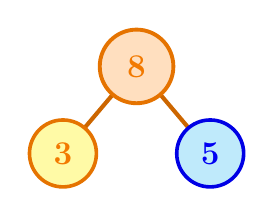
\begin{tikzpicture}[scale=0.85, baseline=(current bounding box.center)]
  \VeSoDoTachGop{0}{0}{8}{3}{5}{orange}
\end{tikzpicture}
\end{center}
\choiceTF
{\True Từ sơ đồ trên ta có phép tính $3 + 5 = 8$.}
{\True Từ sơ đồ trên ta có phép tính $8 - 3 = 5$.}
{Từ sơ đồ trên ta có phép tính $8 - 5 = 2$.}
{\True Từ sơ đồ trên ta có phép tính $8 - 5 = 3$.}
\loigiai{
\begin{itemize}
    \item a) \textbf{Đúng}: $3 + 5 = 8$.
    \item b) \textbf{Đúng}: $8 - 3 = 5$.
    \item c) \textbf{Sai}: $8 - 5 = 3$, không phải bằng $2$.
    \item d) \textbf{Đúng}: $8 - 5 = 3$.
\end{itemize}
}
\end{ex}

% --- CÂU 14 ---
\begin{ex} %[1D3V12]
Quan sát các cặp số có tổng bằng 10 và xét tính đúng sai:
\begin{center}
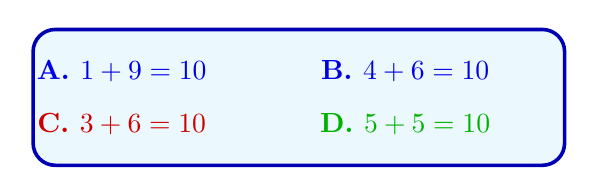
\begin{tikzpicture}[scale=0.75, baseline=(current bounding box.center)]
  \draw[fill=cyan!8, draw=blue!70!black, line width=1.3pt, rounded corners=8pt] (-4.5,-1.15) rectangle (4.5,1.15);
  \node[font=\normalsize\bfseries\color{blue!90!black}] at (-3.0,0.45) {A. $1 + 9 = 10$};
  \node[font=\normalsize\bfseries\color{blue!90!black}] at (1.8,0.45) {B. $4 + 6 = 10$};
  \node[font=\normalsize\bfseries\color{red!80!black}] at (-3.0,-0.45) {C. $3 + 6 = 10$};
  \node[font=\normalsize\bfseries\color{green!70!black}] at (1.8,-0.45) {D. $5 + 5 = 10$};
\end{tikzpicture}
\end{center}
\choiceTF
{\True Cặp số $1$ và $9$ có tổng bằng $10$.}
{\True Cặp số $4$ và $6$ có tổng bằng $10$.}
{Cặp số $3$ và $6$ có tổng bằng $10$.}
{\True Cặp số $5$ và $5$ có tổng bằng $10$.}
\loigiai{
\begin{itemize}
    \item a) \textbf{Đúng}: $1 + 9 = 10$.
    \item b) \textbf{Đúng}: $4 + 6 = 10$.
    \item c) \textbf{Sai}: $3 + 6 = 9$, không bằng 10.
    \item d) \textbf{Đúng}: $5 + 5 = 10$.
\end{itemize}
}
\end{ex}

% =========================================================================
% PHẦN 3: TRẢ LỜI NGẮN (6 CÂU)
% =========================================================================
\textbf{Phần 3. Trả lời ngắn (Quan sát hình vẽ và điền số thích hợp)}
\setcounterpageref{ex}{0}

% --- CÂU 15 ---
\begin{ex} %[1D3H12]
Tính kết quả phép tính: $5 + 5$.
\begin{center}

\begin{tikzpicture}[scale=0.75, baseline=(current bounding box.center)]
  % 2 bàn tay 5 ngón hoặc 2 nhóm 5 chấm tròn
  \foreach \i in {0,1,2,3,4} {
    \fill[red!85!black] (\i*0.8 - 3.6, 0) circle (0.28cm);
  }
  \node[font=\LARGE\bfseries\color{blue!90!black}] at (0,0) {$+$};
  \foreach \i in {0,1,2,3,4} {
    \fill[cyan!80!blue] (\i*0.8 + 0.8, 0) circle (0.28cm);
  }
\end{tikzpicture}
\end{center}
\shortans{10}
\loigiai{
\textbf{Đáp số:} $10$\\
$5 + 5 = 10$.
}
\end{ex}

% --- CÂU 16 ---
\begin{ex} %[1D3H12]
Tính kết quả phép tính: $10 - 6$.
\begin{center}

\begin{tikzpicture}[scale=0.75, baseline=(current bounding box.center)]
  \draw[fill=yellow!20, draw=orange!90!black, line width=1.3pt, rounded corners=6pt] (-3.0,-0.55) rectangle (3.0,0.55);
  \node[font=\Large\bfseries\color{blue!90!black}] at (0,0) {$10 - 6 = ?$};
\end{tikzpicture}
\end{center}
\shortans{4}
\loigiai{
\textbf{Đáp số:} $4$\\
$10 - 6 = 4$.
}
\end{ex}

\newpage
% --- CÂU 17 ---
\begin{ex} %[1D3V12]
Tính giá trị biểu thức: $4 + 6 - 3$.
\begin{center}

\begin{tikzpicture}[scale=0.8, baseline=(current bounding box.center)]
  \draw[fill=cyan!15, draw=blue!80!black, line width=1.3pt, rounded corners=6pt] (-3.2,-0.55) rectangle (3.2,0.55);
  \node[font=\Large\bfseries\color{blue!95!black}] at (0,0) {$4 + 6 - 3 = ?$};
\end{tikzpicture}
\end{center}
\shortans{7}
\loigiai{
\textbf{Đáp số:} $7$\\
$4 + 6 = 10$; $10 - 3 = 7$.
}
\end{ex}

% --- CÂU 18 ---
\begin{ex} %[1D3V12]
Quan sát sơ đồ tách - gộp số 10. Điền số thích hợp vào dấu hỏi chấm:
\begin{center}
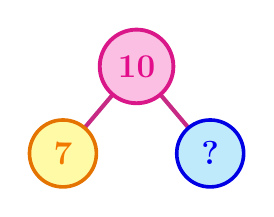
\begin{tikzpicture}[scale=0.85, baseline=(current bounding box.center)]
  \VeSoDoTachGop{0}{0}{10}{7}{?}{magenta}
\end{tikzpicture}
\end{center}
\shortans{3}
\loigiai{
\textbf{Đáp số:} $3$\\
$10 - 7 = 3$.
}
\end{ex}

% --- CÂU 19 ---
\begin{ex} %[1D3V12]
Trong vườn có 10 cây hoa gồm hoa hồng đỏ và hoa cúc vàng. Biết có 6 cây hoa hồng đỏ, hỏi có bao nhiêu cây hoa cúc vàng?
\begin{center}
\begin{tikzpicture}[scale=0.8, baseline=(current bounding box.center)]
  \draw[fill=green!10, draw=green!70!black, line width=1.3pt, rounded corners=8pt] (-4.2,-1.0) rectangle (4.2,1.0);
  % 6 hoa hồng đỏ
  \foreach \i in {0,1,2,3,4,5} {
    \VeBongHoaNho[red!85!black]{\i*0.75 - 3.4}{0.2}
  }
  \node[below=3pt, font=\small\bfseries\color{red!85!black}] at (-1.5,-0.5) {6 hoa hồng};
  
  \draw[dashed, line width=1pt, gray!60] (0.2,-0.75) -- (0.2,0.75);
  
  \node[font=\Large\bfseries\color{orange!90!black}] at (2.2,0.2) {? hoa cúc};
  \node[below=3pt, font=\small\bfseries\color{blue!85!black}] at (2.2,-0.5) {Tổng có 10 cây};
\end{tikzpicture}
\end{center}
\shortans{4}
\loigiai{
\textbf{Đáp số:} $4$\\
$10 - 6 = 4$ cây hoa cúc.
}
\end{ex}

% --- CÂU 20 ---
\begin{ex} %[1D3C12]
Tính nhanh kết quả phép tính: $2 + 5 + 3$.
\begin{center}
\begin{tikzpicture}[scale=0.8, baseline=(current bounding box.center)]
  \draw[fill=yellow!25, draw=orange!90!black, line width=1.3pt, rounded corners=6pt] (-3.5,-0.6) rectangle (3.5,0.6);
  \node[font=\Large\bfseries\color{red!85!black}] at (0,0) {$2 + 5 + 3 = ?$};
  \node[below=4pt, font=\small\bfseries\color{blue!85!black}] at (0,-0.65) {Gợi ý: Gộp $2 + 3 = 5$, sau đó tính $5 + 5$};
\end{tikzpicture}
\end{center}
\shortans{10}
\loigiai{
\textbf{Đáp số:} $10$\\
Tính nhanh: $(2 + 3) + 5 = 5 + 5 = 10$.
}
\end{ex}
